\documentclass[annotation,times,page4]{itmo-student-thesis}
%% Опции пакета:
%% - annotation - если есть, генерируется аннотация, иначе не генерируется
%% - times - делает все шрифтом Times New Roman, требует пакета pscyr.
%% - page4 - начинает нумерацию оглавления с четвертой, а не с третьей страницы
%% Данные пакеты необязательны к использованию в бакалаврских/магистерских
%% Они нужны для иллюстративных целей
%% Начало
\usepackage{tikz}
\usepackage{graphicx}
\usepackage{placeins}
\graphicspath{ {images/} }
\usetikzlibrary{arrows}
\usepackage{filecontents}
\begin{filecontents}{bachelor-thesis.bib}
	@inproceedings{ example-english,
		year        = {2015},
		booktitle   = {Proceedings of IEEE Congress on Evolutionary Computation},
		author      = {Maxim Buzdalov and Anatoly Shalyto},
		title       = {Hard Test Generation for Augmenting Path Maximum Flow 
			Algorithms using Genetic Algorithms: Revisited},
		pages       = {2121-2128},
		langid      = {english}
	}
	
	@article{ example-russian,
		author      = {Виктор Сергеевич Хованский},
		title       = {Генерация тестов для олимпиадных задач по программированию 
			с использованием генетических алгоритмов},
		journal     = {Научно-технический вестник {СПбГУ} {ИТМО}},
		number      = {2(72)},
		year        = {2011},
		pages       = {72-77},
		langid      = {russian}
	}
\end{filecontents}
%% Конец

%% Указываем файл с библиографией.
\addbibresource{bachelor-thesis.bib}

\begin{document}
	
	\studygroup{M3439}
	\title{Инкрементальный адаптивный алгоритм для построения маршрутов по заданным критериям в транспортной сети}
	\author{Хованский В.С.}
	\supervisor{Шалыто А.А.}
	\supervisordegree{канд. техн. наук, доцент}
	\publishyear{2016}
	
	%% Транслируется в "Направление и задача исследований"
	\researchdirections{Целью данной работы является иллюстрация стилевого файла \LaTeX\
		для оформления бакалаврских работ в ИТМО.}
	
	%% Транслируется в "Проектная и исследовательская часть"
	\researchpart{Данная работа является примером оформления бакалаврской работы с использованием стилевого файла
		\texttt{itmo-student-thesis.cls}, разработанного Буздаловым~М.~В. для замены старого комплекта стилевых файлов,
		имеющего хождение на кафедре <<Компьютерные технологии>> Университета ИТМО.}
	
	%% Транслируется в "Экономическая часть"
	\economicpart{Данная работа не предполагает извлечения прямой экономической выгоды 
		из полученных результатов.}
	
	%% Транслируется в "Характеристика вопросов экологии, техники безопасности"
	\ecologypart{Результатом работы является программный продукт, не нарушающий 
		требования экологической безопасности.}
	
	%% Транслируется в "Новизна полученных результатов"
	\novelty{Полученные результаты являются новыми, по крайней мере, ранее существующий стилевой файл
		никоим образом не соответствует ГОСТ, кроме того, он устроен совершенно уродским образом
		и не генерирует титульных страниц и аннотаций.}
	
	%% Транслируется в "Является ли работа продолжением курсовых проектов, есть ли публикации"
	\cwpublications{Работа является продолжением работ над оформлением в \LaTeX\
		кандидатской диссертации и отчетов о НИР.}
	
	%% Транслируется в "Практическая ценность работы. Рекомендации по внедрению"
	\practicalimplications{Результаты, полученные в работе, могут быть использованы как довольно
		удобный способ получить халявное ГОСТ-образное форматирование в своей бакалаврской работе.}
	
	%% Эта команда генерирует титульный лист и аннотацию.
	\makebachelortitle
	
	%% Оглавление
	\tableofcontents
	
	%% Макрос для введения. Совместим со старым стилевиком.
	\startprefacepage
	
	В данном разделе размещается введение.
	
	%% Начало содержательной части.
\chapter{Глава 1. Обзор предметной области}
В данной главе описаны основные определения и определения из области построения маршрутов в теории графов. В первом разделе главы описаны понятия из теории графов. Во втором разделе описаны понятия из формальной области транспортных сетей. В третьем разделе формализуется задача и список требований по поддерживаемым свойствам для построения маршрутов. Четвертый раздел содержит краткое описание основных алгоритмов теории графов для построения путей со сводной таблицей преимуществ и недостатков данных подходов.

\section{Основные определения}
\begin{definition}
Теория графов -- раздел дискретной математики, изучающий свойства графов.
\end{definition}

\begin{definition}
Граф -- это множество вершин(узлов), соединенных ребрами. В строгом определении графом называется такая пара множеств. $G=(E, V)$, где $V$ есть подмножество любого счетного множества, а $E$ -- подмножество $V \times V$.
\end{definition}

\begin{definition}
Маршрут -- это конечная последовательность вершин, в которой каждая вершина (кроме последней) соединена со следующей в последовательности вершиной ребром. Цепью называется маршрут без повторяющихся рёбер. Простой цепью называется маршрут без повторяющихся вершин (откуда следует, что в простой цепи нет повторяющихся рёбер).
\end{definition}

\begin{definition}
Ориентированный маршрут (или путь) -- это конечная последовательность вершин и дуг, в которой каждый элемент инцидентен предыдущему и последующему.
\end{definition}

\begin{definition}
Цикл -- это цепь, в которой первая и последняя вершины совпадают. При этом длиной пути (или цикла) называют число составляющих его ребер. Заметим, что если вершины и являются концами некоторого ребра, то согласно данному определению, последовательность является циклом. Чтобы избежать таких «вырожденных» случаев, вводят следующие понятия.
\end{definition}

\begin{definition}
Транспортное средство -- это совокупность технических систем, предназначенных для перемещений людей и грузов из одного места в другое.
\end{definition}

\begin{definition}
Транспортный узел -- это комплекс транспортных устройств в пункте стыка нескольких видов транспорта, совместно выполняющих операции по обслуживанию транзитных, местных и городских перевозок грузов и пассажиров.
\end{definition}

\begin{definition}
Транспортный рейс --
\end{definition}

\begin{definition}
Транспортная сеть -- это совокупность всех транспортных рейсов, представленных в течение интервала продажи билетов.
\end{definition}

\begin{definition}
Остановка — специально отведенное общественное место, предназначенное для посадки/высадки пассажиров рейсового транспортного средства.
\end{definition}

\begin{definition}
Расписание — 
\end{definition}

\begin{definition}
Мульмодальный маршрут — это конечная последовательность транспортных рейсов, попав на которые в определенные промежутки времени можно добраться от начального транспортного узла до конечного.
\end{definition}

\begin{definition}
Построитель маршрутов — это программный комплекс для обработки внешних поисковых клиентских запросов, имеющий доступ к полному объему данных о расписаниях на всех транспортных узлах и осуществляющий выдачу определенного количества маршрутов в соответствии с поступившими в запросах требованиями. Также в качестве дополнительных возможностей доступно построение фильтров и различной статистики (активные транспортные узлы, активные транспортные рейсы, проходящие через заданный узел).
\end{definition}

\begin{definition}
Клиентское приложение — это любое приложение, которое осуществляет запросы к построителю маршрутов за результатом (маршрутами и фильтрами).
\end{definition}

\section{Виды транспорта и его особенности}
В транспортной сети, в которой будут строиться маршруты, будет существовать только транспорт с конкретным расписанием транспортных рейсов. Таким образом, идет допущение о том, что система сети идеальна и весь транспорт гарантировано совершает остановки в назначенное время. Постановка вспомогательных свойств для построителя маршрутов, которые позволяют сгладить последствия этого допущения будут описаны в следующих главах. Далее идет описание рассматриваемого транспорта.

\subsection{Железнодорожный}
В задаче будут рассматриваться 2 вида железнодорожного транспорта. Во-первых, это будут поезда дальнего следования, у которых небольшое количество рейсов (около $10^5$ в течение интервала продажи билетов). Во-вторых, это будут электрички, которые уже совершают до $10^6$ рейсов за аналогичный промежуток времени.
Транспортными узлами являются железнодорожные станции и вокзалы.

\subsection{Воздушный}
Воздушный транспорт будет представлен только самолетами. При этом количество рейсов около $10^3$, поэтому особый интерес этот случай не представляет. Но стоит отметить, что в большинстве случаев мультимодальный маршрут не будет содержать больше одного воздушного сегмента пути.
Транспортными узлами являются аэропорты.

\subsection{Автомобильный}
Автомобильный транспорт состоит из автобусных междугородних рейсов. Около 95\% таких рейсов совершаются только между соседними городами, что сильно упрощает задачу, но количество все равно большое — $10^6$.
Также в эту категорию входит транспорт в пределах города (или любого крупного населенного пункта), например, такси. Стоит отметить, что в этот вид транспорта можно внести любые другие средства передвижения внутри города, так как в конечном счете это не будет влиять на алгоритм. При этом важно, чтобы у нового транспорта в пределах города имелась возможность рассчитать эвристическое времени передвижения между двумя транспортными узлами, которые относятся к одному населенному пункту. Эту задачу следует решать на основе статистики или с помощью сторонних сервисов, которые умеют анализировать дорожную ситуацию, например, такие сервисы, как 2gis или Яндекс.карты, которые могут оценить время движения на основе карты пробок.
Транспортными узлами являются автобусные остановки и крупные населенные пункты.

\section{Построение маршрутов}
Основная задача, ставящаяся перед построителем маршрутов — построение маршрутов по данным, доступным в его памяти и внешних базах данных, доступных для чтения в конкретный момент времени. На алгоритм построения маршрутов в транспортной сети накладываются следующие условия и ограничениями.

\subsection{Мультимодальность}
Маршруты могут быть мультимодальными, то есть проходить через несколько точек-остановок, содержать пересадки, проходить разными видами транспорта со своими особенностями и т.д.; Это нужно для того, чтобы была возможность добраться из любой точки в любую, где есть хотя бы какой-нибудь транспорт. Вариант пройти пешком небольшой кусок пути тоже доступен внутри крупного населенного пункта также должен быть доступен.
\begin{figure}[!h]
    \centering
    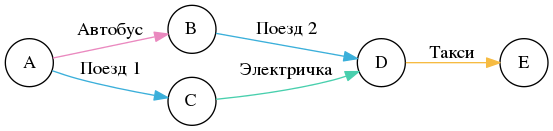
\includegraphics[width=\textwidth]{multimodal_example.png}
    \caption{Несколько мультимодальных маршрутов от точки A до точки E.}\label{fig1}
\end{figure}

\subsection{Временные интервалы}
Маршруты можно строить для определенных интервалов времени. Например, хотим выехать в промежуток с 8-00 до 12-00 утра, а приехать в любой день на следующей неделе, но обязательно после 21-00. Это требуется, чтобы иметь возможность бронировать гостиницу, не отходя от кассы.

\subsection{Инкрементальное построение}
Маршруты требуется строить инкрементально (не все сразу, а только небольшую часть из существующих) из-за того, что возможное количество маршрутов может достигать до 109 между парой крупных населенных пунктов с 3 допустимыми пересадками и интервалом времени в пути равным нескольким дням. Это требуется для конечного клиентского приложения, чтобы можно было организовать страничный показ результатов без полного вычисления всех маршрутов на предыдущих страницах.

\subsection{Адаптивность по времени}
Маршруты могут строиться адаптивно по времени из-за того, что важно время отклика алгоритма, то есть в приоритете время выполнения над показом действительно всех требуемых результатов.

\section{Построение фильтров к доступным маршрутам}
Под фильтром в данном случае понимается предикат, который принимает в качестве аргумента построенный маршрут и возвращает ИСТИНА или ЛОЖЬ в зависимости от того, удовлетворяет ли маршрут критериям поиска, которые задает фильтр.
Таким образом, помимо построения самих маршрутов требуется построить фильтры по доступным маршрутам со следующими условиями.

\subsection{Косвенные признаки}
Из-за того, что маршруты строятся не все сразу, то кроме непосредственно найденных маршрутов существует огромное количество потенциально доступных маршрутов. При этом мы хотим получить к ним доступ по косвенным признаками. Например, это может быть тип транспорта, номер поезда или тип места в самолете (у окна/у туалета/в хвосте). Формально любой параметр доступный в модели данных может стать доступным для фильтрации.
Примечание. Под моделью данных в данном случае подразумевается любой абстрактный объект, который имеет отражение в реальном мире: поезд, самолет, аэропорт и т.д.

\subsection{Осуществление фильтрации}


\subsection{Функциональные зависимости}
Не последнюю роль в фильтрах играют функциональные зависимости, потому что в последствии нужно будет их эффективно показывать без противоречий. Например, тип места «у окна» в купе и каюте относятся к разным типам транспорта и их нельзя объединять. Пример «дерева» функциональный зависимостей для поезда:
\begin{itemize}
    \item Точки отправления и прибытия
    \item Интервалы отправления и прибытия
    \item Вид транспорта:
    \item Поезд:
    \begin{itemize}
	    \item Перевозчик
	    \item Бренд
	    \item Номер
	    \item Тип вагона:
	    \begin{itemize}
	    	\item Купе:
	    	\begin{itemize}
	    		\item Верхнее/нижнее
	    		\item Не у туалета
	    	\end{itemize}
	    	\item Сидячий:
	    	\begin{itemize}
	    		\item У окна/у прохода
	    	\end{itemize}
	    	\item Плацкарт:
	    	\begin{itemize}
	    		\item Верхнее/нижнее
	    		\item Не у туалета
	    		\item Боковое/не боковое
	    	\end{itemize}
	    \end{itemize}
	\end{itemize}
\end{itemize}

Каждый уровень списка зависит от родительского уровня и строго им определяется для того, чтобы исключить ситуации, когда несколько косвенных признаков совпадают уже разных видов транспорта. Например, признак «Перевозчик» у поезда и самолета. Такое разделение необходимо для корректного с точки зрения логики и удобного вывода результата в клиентском приложении.

\section{Сортировка маршрутов}
Маршруты требуется строить в порядке сортировки. В простейшем варианте можно сортировать только построенные маршруты, что не представляет из себя никакой сложности. В сложном варианте маршруты строятся на основе любого предиката сравнения пары маршрутов и выдаются в результат, гарантируя определенный порядок. В рамках данной работы подходит «средний» вариант. Требуется гарантировать определенный порядок построенных маршрутов без пропусков, но предикаты известны заранее. Всего их основных 4 вида:
\begin{enumerate}
    \item Количество пересадок
    \item Время отправления
    \item Время прибытия
    \item Время в пути
\end{enumerate}

Рассмотрим каждый подробнее.

\subsection{Количество пересадок}
Самая простая сортировка в рамках данной работы (или просто сортировка по-умолчанию). Несложно заметить, что количество пересадок будет пропорционально количеству транспорта, который будет включен в мультимодальный маршрут. И если представить каждый отрезок пути на конкретном транспорте отдельным ребром в абстрактном графе, то сортировка будет происходить относительно количества ребер.
\subsection{Время отправления}

\subsection{Время прибытия}

\subsection{Время в пути}

\section{Известные алгоритмы}
\subsection{Алгоритм Дейкстры}
Классический алгоритм для вычисления кратчайших путей в статическом графе $G=(V, E)$ с функцией веса\footnote{Предполагается, что в статическом графе ребра имеют неотрицательные веса. Для общего случая можно использовать алгоритм Беллмана — Форда.} для ребер называется алгоритмом Дейкстры. В частности, алгоритм, разработанный Э. Дейкстрой, решает проблему нахождения кратчайших маршрутов от единственной стартовой вершины $s$ до всех остальных вершин в графе $G$. Алгоритм поддерживает для каждой вершины $u$ метку $\delta(u)$ с предварительным расстояние от $s$ до $u$. Каждая вершина может находится в одном из следующих состояниях: нерассмотренная, рассмотренная, посещенная. 

Изначально только вершина $s$ считается рассмотренной с $\delta(s)=0$ и все остальные вершины $u$ являются нерассмотренными с $\delta(u)=\infty$.

На каждом шаге вершина $u$ с минимальной $\delta(u)$ извлекается и удаляется из приоритетной очереди $Q$. Будет говорить, что вершина посещена, так как теперь известно, что $\delta(u)$ -- кратчайшее расстояние. Все исходящие ребра $(u, v)$ посещенной вершины релаксируются, то есть сравнивается кратчайшее расстояние от $s$ через $u$ до вершины $v$ с предварительным расстоянием $\delta(v)$. Если оно меньше, то мы обновляет $\delta(v)$ и $v$ в приоритетной очереди $Q$. Стоит заметить, что такое обновление для нее это либо операции вставки, если вершина рассмотрена, либо операция уменьшения ключа в противном случае. Алгоритм заканчивает работу только тогда, когда очередь становится пустой. Это произойдет после $n$ шагов, где $n$ -- это количество вершин в графе $G$.

В приведенном ниже псевдокоде видно, что иногда мы не посещаем все вершины в графе. Это происходит из-за того, что либо такие вершины недостижимы из $s$, либо очередь становится пустой раньше, чем мы доходим до такой вершины. Для того, чтобы избежать инициализации алгоритма за $O(n)$ при последовательных вызовах, можно сохранять посещенные вершины и обновлять их значения $\delta$ после конца алгоритма. Таким образом, асимптотика алгоритма зависит только от количества посещенных вершин и релаксируемых ребер, а не от $n$. 

\begin{algorithm}[!h]
	\caption{Алгоритм Дейкстры}\label{lst1}
	\begin{algorithmic}
		\Function{Dijkstra}{$s$}
		\State $\delta = \left\{\infty, ..., \infty\right\}$ \Comment{предварительные расстояния}
		\State $\delta(s) = 0$ \Comment{поиск начинается из вершины $s$}
		\State $Q.update(0, s)$ \Comment{приоритетная очередь}
		\While{$Q \neq \emptyset $}
			\State $(_, u)$ = Q.deleteMin() \Comment{посещаем $u$}
			\For{$ e = (u, v) \in E$} \Comment{релаксируем ребра}
				\If{$ \delta(u) + c(e) < \delta(v) $}
					\State $delta(v) = \delta(u) + c(e)$
					\State $Q.update(\delta(v), v)$
				\EndIf
			\EndFor
		\EndWhile
		\EndFunction
	\end{algorithmic}
\end{algorithm}

Алгоритм Дейкстры использует максимум $n$ операций вставки в приоритетную очередь, $n$ удалений и $m$ операций уменьшения ключа, обеспечивая таким образом асимптотику $O(m + n \log n)$ при использовании Фибоначчиевой кучи.

\begin{figure}[!h]
	\centering
	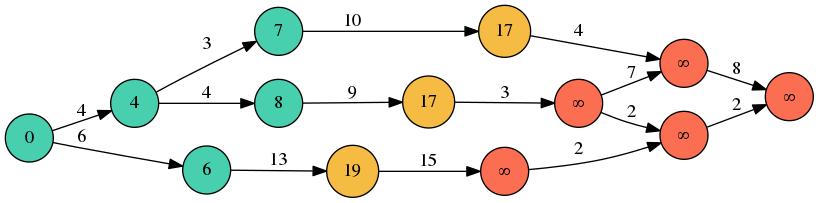
\includegraphics[width=\textwidth]{dijkstra_example.png}
	\caption{Состояние алгоритма Дейкстры после посещения 5 вершин. Посещенные - зеленые, рассмотренные - желтые, нерассмотренные - красные.}\label{fig1}
\end{figure}


\subsection{Алгоритм Йена}
Алгоритм Йена находит $k$ путей без циклов от единственной стартовой вершины $s$ до конечной вершины $t$ в статичном графе. Разработанный Йеном алгоритм предполагает, что в его основе будет лежать любой другой алгоритм поиска кратчайшего пути, например, его основой может послужить алгоритм Дейкстры. Идея основана на том, что можно построить изначально кратчайший путь и потом на основе этого пути искать отклонения, чтобы построить следующий. Каждая $k$ итерация будет искать отклонения от кратчайших путей, полученных на $k-1$ итерациях.

\section{Таблицы}

В качестве примера таблицы приведена таблица~\ref{tab1}.

\begin{table}[!h]
\caption{Таблица умножения (фрагмент)}\label{tab1}
\centering
\begin{tabular}{|*{18}{c|}}\hline
-- & 1 & 2 & 3 & 4 & 5 & 6 & 7 & 8 & 9 & 10 & 11 & 12 & 13 & 14 & 15 & 16 & 17 \\\hline
1  & 1 & 2 & 3 & 4 & 5 & 6 & 7 & 8 & 9 & 10 & 11 & 12 & 13 & 14 & 15 & 16 & 17 \\\hline
2  & 2 & 4 & 6 & 8 & 10 & 12 & 14 & 16 & 18 & 20 & 22 & 24 & 26 & 28 & 30 & 32 & 34 \\\hline
3  & 3 & 6 & 9 & 12 & 15 & 18 & 21 & 24 & 27 & 30 & 33 & 36 & 39 & 42 & 45 & 48 & 51 \\\hline
4  & 4 & 8 & 12 & 16 & 20 & 24 & 28 & 32 & 36 & 40 & 44 & 48 & 52 & 56 & 60 & 64 & 68 \\\hline
\end{tabular}
\end{table}

Есть еще такое окружение \texttt{tabu}, его можно аккуратно растянуть на всю страницу.
Приведем пример (таблица~\ref{tab2}).

\begin{table}[!h]
\caption{Таблица умножения с помощью \texttt{tabu} (фрагмент)}\label{tab2}
\centering
\begin{tabu}{|*{18}{X[c]|}}\hline
-- & 1 & 2 & 3 & 4 & 5 & 6 & 7 & 8 & 9 & 10 & 11 & 12 & 13 & 14 & 15 & 16 & 17 \\\hline
1  & 1 & 2 & 3 & 4 & 5 & 6 & 7 & 8 & 9 & 10 & 11 & 12 & 13 & 14 & 15 & 16 & 17 \\\hline
2  & 2 & 4 & 6 & 8 & 10 & 12 & 14 & 16 & 18 & 20 & 22 & 24 & 26 & 28 & 30 & 32 & 34 \\\hline
3  & 3 & 6 & 9 & 12 & 15 & 18 & 21 & 24 & 27 & 30 & 33 & 36 & 39 & 42 & 45 & 48 & 51 \\\hline
4  & 4 & 8 & 12 & 16 & 20 & 24 & 28 & 32 & 36 & 40 & 44 & 48 & 52 & 56 & 60 & 64 & 68 \\\hline
\end{tabu}
\end{table}

\section{Рисунки}

Пример рисунка (c помощью \texttt{TikZ}) приведен на рисунке~\ref{fig1}. Под \texttt{pdflatex} можно также
использовать \texttt{*.jpg}, \texttt{*.png} и даже \texttt{*.pdf}, под \texttt{latex} можно использовать
Metapost. Последний можно использовать и под \texttt{pdflatex}, для чего в стилевике продекларированы
номера картинок от~1 до~20.

\begin{figure}[!h]
\caption{Пример рисунка}\label{fig1}
\centering
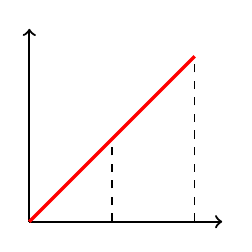
\begin{tikzpicture}[scale=0.7]
\draw[thick,->] (0,0)--(3.5,0);
\draw[thick,->] (0,0)--(0,3.5);
\draw[very thick, red] (0,0)--(3,3);
\draw[dashed] (3,0)--(3,3);
\draw[dashed] (1.5,0)--(1.5,1.5);
\end{tikzpicture}
\end{figure}

\section{Листинги}

В работах студентов кафедры <<Компьютерные технологии>> часто встречаются различные листинги. Листинги бывают
двух основных видов~--- исходный код и псевдокод. Первый оформляется с помощью окружения \texttt{lstlisting}
из пакета \texttt{listings}, который уже включается в стилевике и немного настроен. Пример Hello World на Java
приведен на листинге~\ref{lst1}.

\begin{lstlisting}[float=!h,caption={Пример исходного кода на Java},label={lst1}]
public class HelloWorld {
	public static void main(String[] args) {
		System.out.println("Hello, world!");
	}
}
\end{lstlisting}

Псевдокод можно оформлять с помощью разных пакетов. В данном стилевике включается пакет \texttt{algorithmicx}.
Сам по себе он не генерирует флоатов, поэтому для них используется пакет \texttt{algorithm}.
Пример их совместного использования приведен на листинге~\ref{lst2}. Обратите внимание, что флоаты разные, а 
нумерация~--- общая!

\begin{algorithm}[!h]
\caption{Пример псевдокода}\label{lst2}
\begin{algorithmic}
	\Function{IsPrime}{$N$}
		\For{$t \gets [2; \lfloor\sqrt{N}\rfloor]$}
			\If{$N \bmod t = 0$}
				\State\Return \textsc{false}
			\EndIf
		\EndFor
		\State\Return \textsc{true}
	\EndFunction
\end{algorithmic}
\end{algorithm}

Наконец, листинги из \texttt{listings} тоже можно подвешивать с помощью \texttt{algorithm},
пример на листинге~\ref{lst3}.

\begin{algorithm}[!h]
\caption{Исходный код и флоат \texttt{algorithm}}\label{lst3}
\begin{lstlisting}
public class HelloWorld {
	public static void main(String[] args) {
		System.out.println("Hello, world!");
	}
}
\end{lstlisting}
\end{algorithm}

	\chapter{Алгоритм построения маршрутов}

\section{Модели данных}
В этом разделе будут описаны 3 способа представления данных о транспортной системе в виде графа, на котором впоследствии будут применятся алгоритмы для построения маршрутов и доступ к которому будет иметь построитель маршрутов.
\subsection{Статичный граф}
В статичном случае каждое ребро взвешенно функцией $c:E \rightarrow R$, и не имеет параллельных ребер. Для каждого ребра $e=(u, v)$ будем писать иногда $c(u, v)$ вместо $c(e)$. Будем называть такой граф простым взвешенным. Вес ребра можно интерпретировать как среднее время движения, требуемое на преодоление сегмента дороги, или как физическую длину. Длина пути $P$ в таком случае равна $c(P)=\sum_{i=1}^{k}c(e_i)$. Путь $P^*$ будет является кратчайшим в том случае, если не существует другого пути $P'$ с такой же стартовой и конечной вершинами, что и у пути $P^*$, такого, что $c(P')<c(P^*)$.

Можно построить граф транспортных рейсов, который будет соответствовать данному случаю. Для этого возьмем на вершину графа транспортный узел, а движение транспорта от одного транспортного узла до другого -- за ребро. За вес ребра будет принята длина сегмента пути, так как она не меняется с течением времени. Далее на таком графе можно применить алгоритм Йена и найти $k$ путей.

К сожалению, такой подход имеет ряд существенных минусов. Во-первых, будет доступна только одна естественная сортировка -- по количеству пересадок, так как в данном случае это будет просто количество ребер. Во-вторых, поддержка временных интервалов потребует дополнительных вызовов алгоритма для того, чтобы гарантированно получить те маршруты, которых попадают в определенные временные границы. В-третьих, это размер графа, который зависит от количества остановок каждого транспорта за период даты продаж.

\begin{figure}[!h]
	\centering
	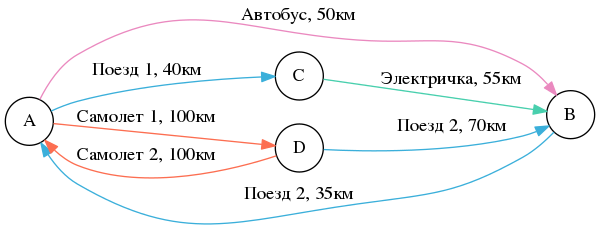
\includegraphics[width=\textwidth]{static_graph_example.png}
	\caption{Статичный граф с 4 городами и 6 транспортами}\label{fig3}
\end{figure}
\FloatBarrier

\subsection{Граф расписаний}
Традиционно расписания представляются множеством поездов (автобусов, самолетов и т.д.). Каждый поезд посещает последовательность станций (автобусных остановок, аэропортов и т.д.). Для каждой станции, за исключением последней, расписание включает в себя время отбытия, и для каждой станции, за исключением первой, включает в себя время прибытия, как показано в таблице:

Для того, чтобы была возможность математически определить связи, состоящие из нескольких поездов, мы разделим их в элементарные связи. Более формально, мы имеет множество станций $B$, множество остановок $Z_S$ на каждой станции $S \in B$ и множество элементарных связей $C$, чьи элементы $c$ являются кортежами вида $c=\{Z_d,Z_a,S_d,S_a,\tau_d,\tau_d\}$. Такой кортеж интерпретируется как поезд, который отправляется со станции $S_d$ со временем отбытия $\tau_d$ после остановки $Z_d$ и затем следующую остановку $Z_a$ на станции $S_a$ с временем прибытия $\tau_a$.

\begin{definition}
	Длительность элементарной связи $c$ определяется как $d(c)=\tau_a(c)-\tau_d(c)$.
\end{definition}

Для моделирования более реалистичных маршрутов в данном графе вес ребра будет зависеть от длительности сегмента пути
\subsection{Граф рейсов}


\section{Построение маршрутов}

\subsection{Дополнение временных интервалов}

\section{Построение фильтров}

\subsection{Косвенные признаки}

\subsection{Осуществление фильтрации}

\subsection{Функциональные зависимости}

\subsection{"Белые" и "черные" фильтры}

\section{Сортировка маршрутов}

\subsection{Количество пересадок}

\subsection{Время прибытия}

\subsection{Время отправления}

\subsection{Время в пути}
Листинг~\ref{lst4} должен иметь номер 4.

\begin{algorithm}[!h]
\caption{Исходный код и флоат \texttt{algorithm}}\label{lst4}
\begin{lstlisting}
public class HelloWorld {
	public static void main(String[] args) {
		System.out.println("Hello, world!");
	}
}
\end{lstlisting}
\end{algorithm}

Рисунок~\ref{fig2} должен иметь номер 2.

\begin{figure}[!h]
\caption{Пример рисунка}\label{fig2}
\centering
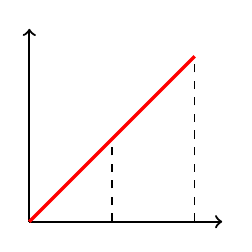
\begin{tikzpicture}[scale=0.7]
\draw[thick,->] (0,0)--(3.5,0);
\draw[thick,->] (0,0)--(0,3.5);
\draw[very thick, red] (0,0)--(3,3);
\draw[dashed] (3,0)--(3,3);
\draw[dashed] (1.5,0)--(1.5,1.5);
\end{tikzpicture}
\end{figure}

Таблица~\ref{tab3} должна иметь номер 3.

\begin{table}[!h]
\caption{Таблица умножения с помощью \texttt{tabu} (фрагмент)}\label{tab3}
\centering
\begin{tabu}{|*{18}{X[c]|}}\hline
-- & 1 & 2 & 3 & 4 & 5 & 6 & 7 & 8 & 9 & 10 & 11 & 12 & 13 & 14 & 15 & 16 & 17 \\\hline
1  & 1 & 2 & 3 & 4 & 5 & 6 & 7 & 8 & 9 & 10 & 11 & 12 & 13 & 14 & 15 & 16 & 17 \\\hline
2  & 2 & 4 & 6 & 8 & 10 & 12 & 14 & 16 & 18 & 20 & 22 & 24 & 26 & 28 & 30 & 32 & 34 \\\hline
3  & 3 & 6 & 9 & 12 & 15 & 18 & 21 & 24 & 27 & 30 & 33 & 36 & 39 & 42 & 45 & 48 & 51 \\\hline
4  & 4 & 8 & 12 & 16 & 20 & 24 & 28 & 32 & 36 & 40 & 44 & 48 & 52 & 56 & 60 & 64 & 68 \\\hline
\end{tabu}
\end{table}

\chapterconclusion

В конце каждой главы желательно делать выводы. Вывод по данной главе~--- нумерация работает корректно, ура!
	\chapter{Детали реализации и тестирование}
В данной главе будут описаны некоторые интересные детали реализации описанных ранее алгоритмов. Во многом аппаратная часть определила подходы, которые использовались при теоретическом исследовании. Все перечисленное было реализовано в виде программных сервисов на языке Java~8.
\section{Работа с базой данных}
Исходя из размера всей транспортной сети, в которую входит информация об узлах, рейсах и расписаниях, не сложно заметить, что её нельзя уместить целиком в оперативной памяти и поэтому нужно использовать эффективное хранение информации -- базу данных. В данной работе была использована VoltDB.
\subsection{Особенности базы данных}
VoltDB - это ACID-совместимая реляционная СУБД, которая использует архитектуру shared nothing architecture. Она опирается на:
\begin{itemize}
	\item горизонтальную разбивку данных (каждый кластер хранит только свою порцию данных) вплоть до отдельного аппаратного потока;
	\item синхронную репликацию данных между всеми обработчиками одного кластера (для обеспечения высокой доступности);
	\item сочетание непрерывных снимков и журнала выполненных команд для обеспечения надежности данных (при восстановлении после сбоя).
\end{itemize}
VoltDB является in-memory СУБД, то есть старается преимущественно держать данные в оперативной памяти сервера, такой подход имеет ряд преимуществ: резко сокращается время отклика и становится проще репликация данных.
\subsection{Персистентные модели данных}
К сожалению, VoltDB поддерживает не все возможности обычных SQL СУБД, поэтому для версионности моделей и хранения истории данных, работа с ней происходит в Key-Value подходе, где ключом является любой комбинированный объект, состоящих из примитивных типов, а значением -- сериализованный Java-объект. Вместо стандартной сериализации используется библиотека Protostuff, которая имеет больше возможностей по сжатию и эффективному хранению данных.

Так как база данных почти полностью написана на Java, хранит объекты Java и предоставляет драйвер на том же языке, то ради повышения производительности объекты стоит сделать персистетными (иммутабельными), чтобы исключить блокировки. Это позволит работать с базой множеству отдельных потоков, исключая траты ресурсов на синхронизацию. 
\subsubsection{Транспорт}
Каждая реальная модель данных разделяется на абстрактную модель Model, в которой хранятся данные, и сущность из базы данных Entity, в которой хранится идентификатор (ID) и номер версии. База данных позволяет работать с сущностями посредством получения текущей версии и изменения модели, которую можно записать в сущность с автоматическим поднятием версии. При этом объект может либо блокироваться на момент обновления, либо работать без блокировок и использовать обновление отдельных полей.
\subsubsection{Остановки и пересадки}
В данный момент нельзя не сказать про очень важное требование к системе -- каждое значение в базе данных не должно занимать больше 1 Мбайт, это исходит из ограничений на размер результата базы данных и особенностей её репликаций, таким образом оно сильно усложняет возможность хранения множеств $T_d(s)$ и $T_a(s)$, доступных по ключу $s$. На данном этапе требуемая память для 1 сущности:
\begin{table}[!h]
	\caption{Базовый расход памяти на 1 сущность.}\label{tab3}
	\centering
	\begin{tabu}{|*{3}{X[c]|}}\hline
		Количество остановок & Занимаемая память (Плотно), Мбайт & Занимаемая память (Нормально), Мбайт \\\hline
		100  & 0.052 & 0.04\\\hline
		1000  & 0.52 & 0.48\\\hline
		10000  & 5.27 & 4.84\\\hline
		100000  & 53.1 & 48.78\\\hline
	\end{tabu}
\end{table}

Плотным вариантом считаются некоторые вокзалы крупных городов, где временные промежутки между события прибытия и отбытия исчисляются в минутах. Для начала ради уменьшения памяти разделим элементарные остановки на 2 типа:
\begin{itemize}
	\item \textbf{Облегченные остановки}. Они будут храниться во множествах $T_d(s)$ и $T_a(s)$ и соответствовать событиям отправления и прибытия на станцию $s$. Содержать будут только номер и ссылку на транспортный рейс.
	\item \textbf{Полные остановки}. В момент получения облегченные остановки будут можно дополнить до полных, так как в тот момент уже будет известна станция и время.
\end{itemize}

\begin{table}[!h]
	\caption{Расход памяти на 1 сущность (Без дублирования)}\label{tab3}
	\centering
	\begin{tabu}{|*{3}{X[c]|}}\hline
		Количество остановок & Занимаемая память (Плотно), Мбайт & Занимаемая память (Нормально), Мбайт \\\hline
		100  & 0.04 & 0.04\\\hline
		1000  & 0.36 & 0.4\\\hline
		10000  & 3.68 & 4.08\\\hline
		100000  & 37.29 & 41.19\\\hline
	\end{tabu}
\end{table}

В данной работе оптимальным вариант решения этой проблемы оказалось разделение этих множеств на более мелкие. Рассмотрим подробнее, что из себя представляет, например, множество $T_d(s)$. В нем хранятся элементарные остановки, которые содержат номер, станцию, транспортный рейс и время. Учитывая, что рейсы повторяются на станции достаточно редко, то разобьем множества по времени. Для этого приведен время в нормализованный вид и переведем в номер. Например, можно из времени убрать часы, минуты и более мелкие величины, то есть извлечь только дату, а уже её перевести в unix-time\footnote{Определяется как количество секунд, прошедших с полуночи (00:00:00 UTC) 1 января 1970 года. В нашем случае можно уменьшить ещё в 3600 раз.}, который будет являться номером. Тогда все множества разобьются на страницы, которые будут хранить только часть элементарных облегченных остановок.

\begin{figure}[!h]
	\centering
	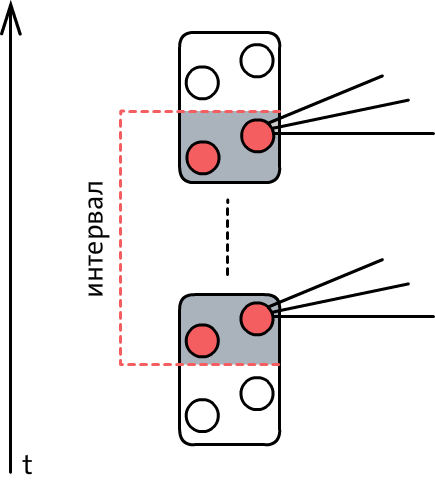
\includegraphics[width=0.5\textwidth]{schedule_pages.png}
	\caption{Страницы элементарных остановок с выходящими сегментами}\label{fig1}
\end{figure}

В результате ряда тестов и исследования методов сериализации в Java было обнаружено, что параметризованные сущности (Generics) сильно влияют на количество памяти после сериализациии. Таким образом, было решено полностью от них избавиться, прописав везде конкретные типы. Также пришлось отказаться от наиболее эффективной структуры данных для получения элементарных остановок в пределах указанного времени java.util.TreeMap, так как её стандартная реализация избыточно хранит большое количество ссылок, а также не поддерживает хранение множества значений для одного ключа (несколько поездов могут отбыть или прибыть в одно и тоже время с точностью до минуты). Наиболее компактной структурной для хранения одной страницы элементарных остановок оказался обычный java.util.ArrayList для пар время-остановка.

\begin{table}[!h]
	\caption{Оптимизированный расход памяти на 1 сущность.}\label{tab3}
	\centering
	\begin{tabu}{|*{3}{X[c]|}}\hline
		Количество остановок & Занимаемая память (Плотно), Мбайт & Занимаемая память (Нормально), Мбайт \\\hline
		100  & 0.01 & 0.01\\\hline
		1000  & 0.07 & 0.08\\\hline
		10000  & 0.71 & 0.87\\\hline
		100000  & 7.14 & 8.69\\\hline
	\end{tabu}
\end{table}

В результате мы может сохранять до 10000 остановок на одну страницу, этого достаточно для всех крупных вокзалов. Обновление страниц будет происходить не часто, поэтому его можно производить с полным копированием данных каждой обновляемой страницы.
\subsection{Кэши}
Зачем это нужно? Конечная система или построитель маршрутов будет географически распределен, база данных будет почти всегда находится физически в другом месте, а требоваться модели будут с различной регулярностью и актуальностью. Поэтому в построитель маршрутов будет добавлено несколько видов кэшей для ускорения работы.

Во-первых, мы добавим кэш для моделей данных. В нем для каждого типа объекта будет храниться его срок годности или частота, с которой его следует обновлять напрямую из базы данных.

Во-вторых, будет добавлен кэш для запросов $q = (s_d, t_d, s_a, t_a, k)$, где для каждого запроса $q$ будет сформирован на основе $s_d$ и $s_a$ уникальный ID, по которому можно будет сохранять результат фазы обхода, то есть множества сегментов и состояний построения. К сожалению, объем памяти построителя маршрутов и клиентского приложения сильно ограничены (для серверной конфигурации), поэтому кэш нужно ограничить по количеству запросов или памяти. Для такой задачи прекрасно подойдет LRU-кэш, то есть кэш основанный на алгоритме кэширования, при котором происходит вытеснение давно неиспользуемых запросов.
\section{Генерация карт транспортных сетей}
Для сравнения и тестирования различных алгоритмов построения маршрутов требуются данные. К сожалению, невозможно выгрузить реальные данные из закрытой системы, а также запустить на идентичных данных разные алгоритмы (данные постоянно меняются), поэтому для тестирования понадобятся дополнительные инструменты. Одним из таким инструментов будет процедурный генератор естественных транспортных сетей.

\begin{figure}[!h]
	\centering
	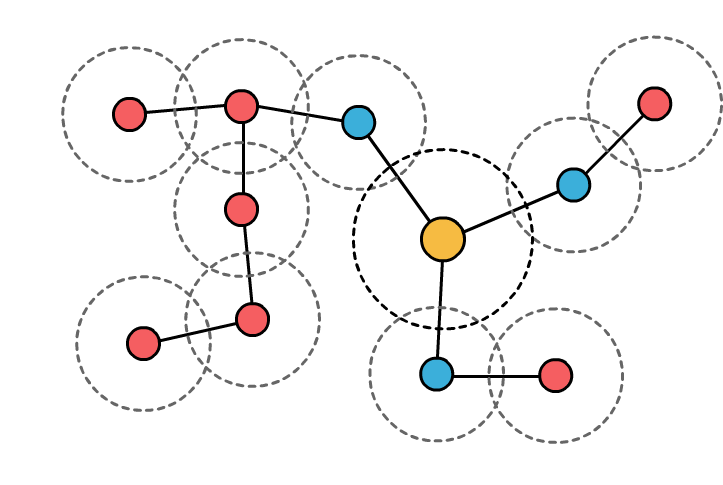
\includegraphics[width=0.9\textwidth]{transport_network.png}
	\caption{Сгенерированная абстрактная транспортная сеть с 1 городом и 3 вокзалами.}\label{fig1}
\end{figure}

Первым делом сгенерируем координаты транспортных узлов. В данном случае можно воспользоваться обычным равномерным псевдослучайным генератором чисел в области ограниченной некоторой кривой. Далее случайным образом выбираются типы транспортных узлов и их признаки из доступного множества признаков.

\subsection{Генерация транспортных рейсов}
Прокладка естественных маршрутов.
\subsection{Генерация центральных узлов}
Генерация точек-городов.

\FloatBarrier
\section{Результаты тестирования}
Время запроса с 10с до 2с, прикрепить 3 графика. Сравнение со старой системой, сравнение с Йеном.

\chapterconclusion
Все сделано и работает. Скорость работы возросла, новые функции появились. Покрыто интеграционными и авто тестами.

	
	%% Макрос для заключения. Совместим со старым стилевиком.
	\startconclusionpage
	
	В данном разделе размещается заключение.
	
	%% Обратите внимание на heading. Без него тоже работает, но название будет другим.
	\printbibliography[heading=trueHeading]
	
	%% После этой команды chapter будет генерировать приложения, нумерованные русскими буквами.
	%% \startappendices из старого стилевика будет делать то же самое
	\appendix
	
	\chapter{Пример приложения}
	
\end{document}